\documentclass[12pt]{article}

\usepackage{amsmath}
\usepackage{array}
\usepackage{caption}
\usepackage[top=1in, bottom=1in, left=0.75in, right=0.75in]{geometry}
\usepackage{graphicx}
\usepackage[colorlinks=true, allcolors=blue]{hyperref}
\usepackage[utf8]{inputenc}
\usepackage{multirow}
\usepackage{pdfpages}
\usepackage[section]{placeins}

\graphicspath{{./figures/}}

\begin{document}

\begin{titlepage}
    \begin{center} \LARGE
        \vspace*{1.5in}

        ECE 272 Lab 2

        Fall 2018

        \vfill

        Adders on an FPGA

        Phi Luu

        \vfill

        October 8\textsuperscript{th}, 2018

        Grading TA: Edgar Perez

        Lab Partner: Benjamin Geyer

        \vspace{1.5in}
    \end{center}
\end{titlepage}

%%%%%%%%%%%%%%%%%%%%%%%%%%%%%%%%%%%%%%%%%%%%%%%%%%%%%%%%%%%%%%%%%%%%%%%%%%%%%%%%
% Introduction
%%%%%%%%%%%%%%%%%%%%%%%%%%%%%%%%%%%%%%%%%%%%%%%%%%%%%%%%%%%%%%%%%%%%%%%%%%%%%%%%
\section{Introduction}

This lab focuses on the logic level of computer arithmetic and a critical component of processors---called the \textit{Arithmetic Logic Unit} (ALU)---that performs arithmetic operations. This lab shows how to implement a system of adders to perform and demonstrate additions of two 4-bit binary numbers using combinational logic design.

There are three main ways of implementing multi-bit adders from combinational logic: ripple-carry, carry-lookahead, and carry-save. There is a tradeoff between speed and size of the three methods. Ripple-carry adders are the slowest but smallest, and carry-save adders are the fastest but biggest. The logic designer can choose between the three depending on the situation. Because the ripple-carry adder is easy to understand and implement, it will be the main focus on this lab.

We will also learn how to use Quartus Prime to design a ripple-carry adder from scratch (logic gates and wires), make the adder itself as a logic symbol, and then use that symbol to perform 4-bit binary addition operations.

%%%%%%%%%%%%%%%%%%%%%%%%%%%%%%%%%%%%%%%%%%%%%%%%%%%%%%%%%%%%%%%%%%%%%%%%%%%%%%%%
% Design
%%%%%%%%%%%%%%%%%%%%%%%%%%%%%%%%%%%%%%%%%%%%%%%%%%%%%%%%%%%%%%%%%%%%%%%%%%%%%%%%
\section{Design}

A ripple-carry takes in three inputs---\textbf{operand1}, \textbf{operand2}, and the \textbf{carry-in}---and produces two outputs, the \textbf{sum} and the \textbf{carry-out}, as sketched in Figure~\ref{figure:1} below:

\begin{figure}[h]
    \centering
    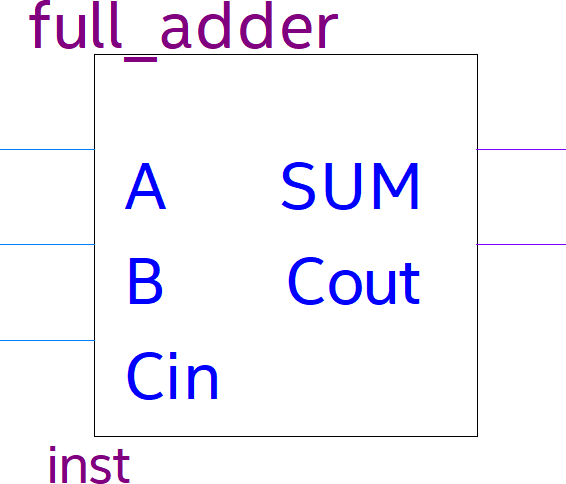
\includegraphics[width=0.5\textwidth]{full_adder_layout.png}
    \caption{The pin layout of a full ripple-carry adder for $A + B$}
    \label{figure:1}
\end{figure}

The carry-in works similarly to when we carry the numbers when adding decimals together. If the value of the carry-in is $1$, then the addition on the more significant column will increase by $1$. If the next column's addition result is already $1$ before adding the carry-in, then its value will circle back to $0$ and continue carrying the $1$ to the more significant column and so on.

\newpage

The block diagram showing the structure of the implementation is as follows:

\begin{figure}[h]
    \centering
    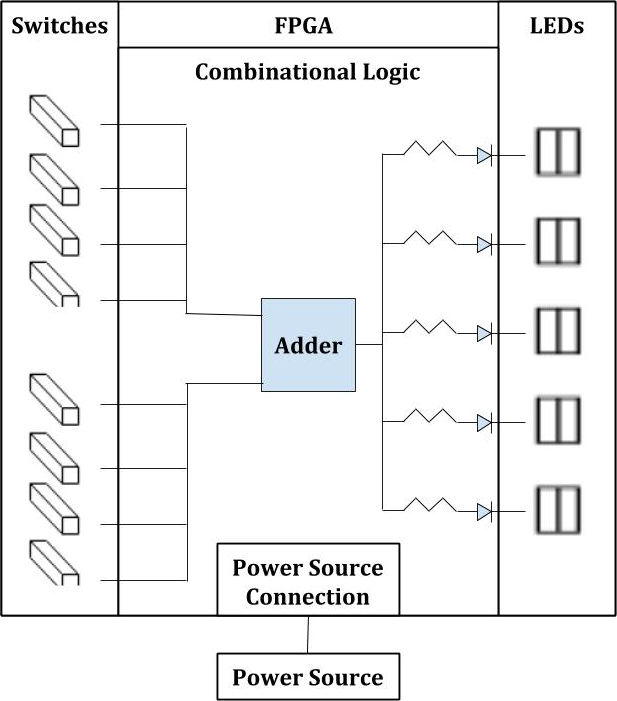
\includegraphics[width=0.5\textwidth]{block_diagram.png}
    \caption{The block diagram showing the connections between the switches, the FPGA, and the LEDs in a 4-bit binary adder implementation}
\end{figure}

Since the circuit takes in two 4-bit binary numbers as operands, there are four pairs of 2-bit inputs---one bit from the first operand and the other from the second operand. Each ripple-carry adder will take in one of the pairs described earlier and return the carry-out with the sum. The adder that ties to the addition of the \textbf{least significant} bits of the two binary numbers will have \textbf{no carry-in value} ($C_{in0} = 0$). Similarly, the adder that ties to the addition of the \textbf{most significant} bits of the two binary numbers will have its \textbf{carry-out connected to the output}, as in some cases the result can be a 5-bit binary number. Finally, the remaining adders will connect to each other in the same way as follows: \textbf{the carry-out of the less significant adders connects to the carry-in of the more significant adders}.

A picture is worth a thousand words. Therefore, the schematic of the internal structure of a ripple-carry adder and the schematic of the 4-bit binary addition circuit are shown in Figures~\ref{figure:2} and~\ref{figure:3}, respectively.

\begin{figure}
    \centering
    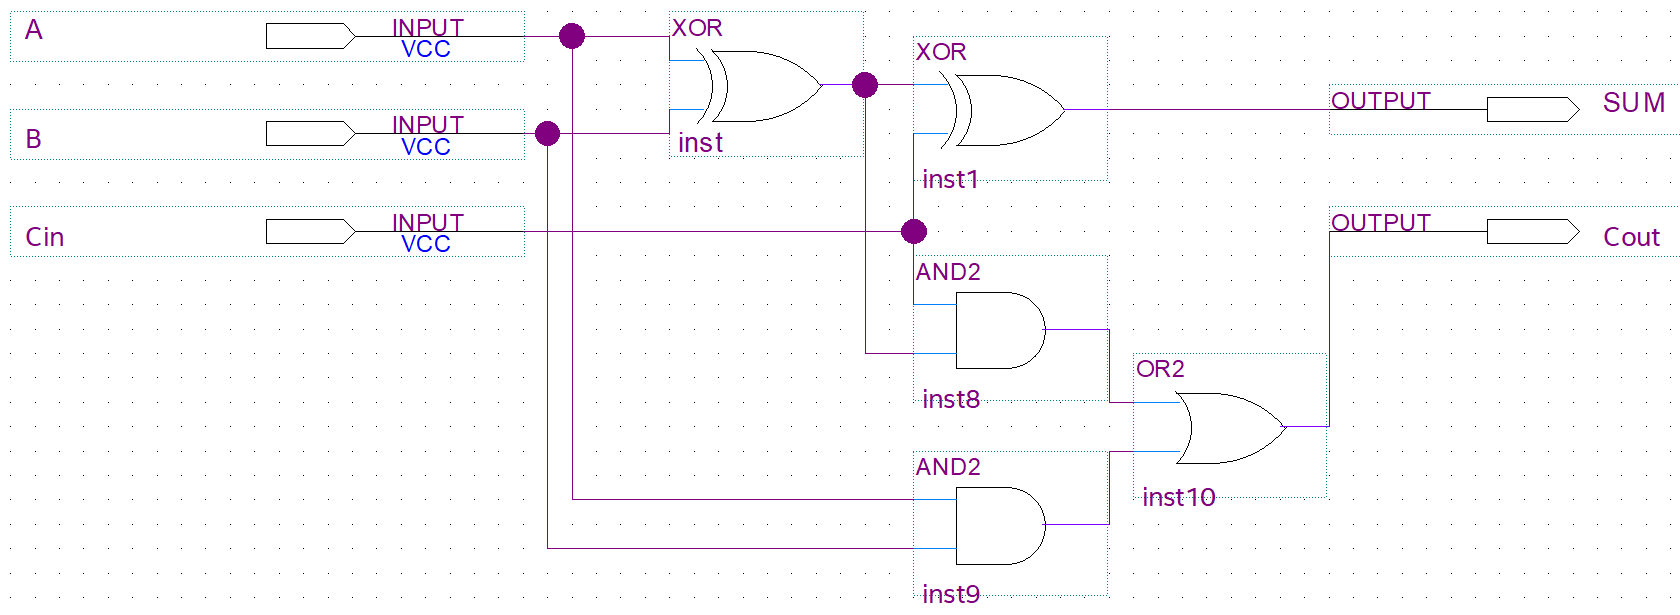
\includegraphics[width=\textwidth]{full_adder_schematic.png}
    \caption{The internal logic-level structure of a full ripple-carry adder}
    \label{figure:2}
\end{figure}

\begin{figure}
    \centering
    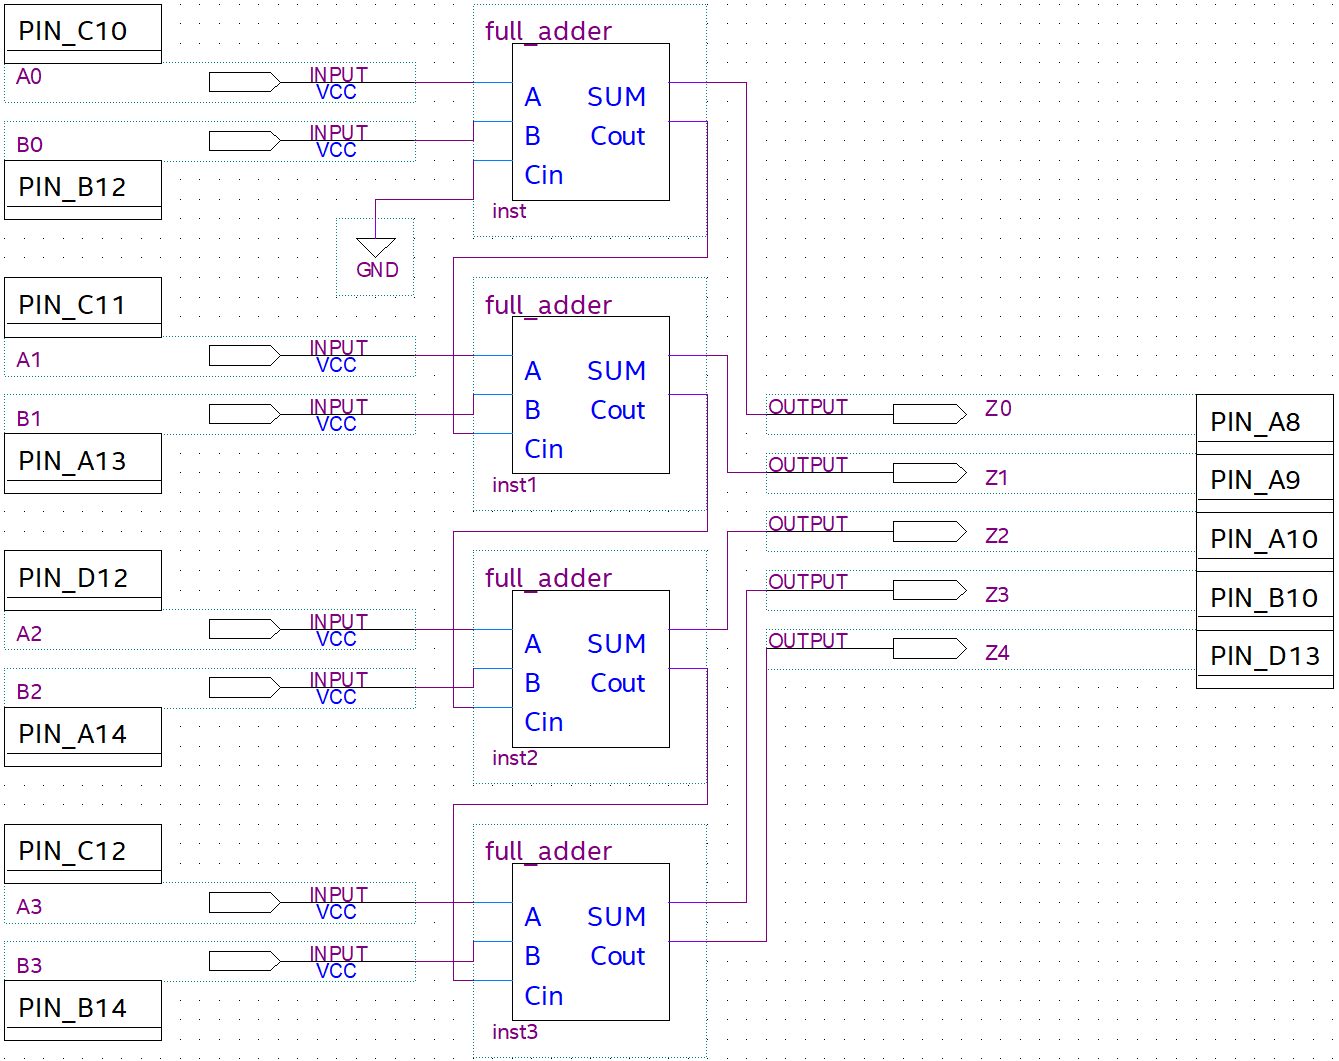
\includegraphics[width=0.9\textwidth]{schematic.png}
    \caption{The schematic of the main circuit}
    \label{figure:3}
\end{figure}

\newpage

Using Figure~\ref{figure:2}, the sum $SUM$ and the carry-out $C_{out}$ of a ripple-adder with operand $A$, operand $B$, and carry-in $C_{in}$ are expressed in the following sum-of-products forms in Equations~\ref{equation:1} and~\ref{equation:2}:

\begin{equation} \label{equation:1}
    SUM = A \oplus B \oplus C_{in}
\end{equation}

\begin{equation} \label{equation:2}
    C_{out} = AB + AC_{in} \oplus BC_{in}
\end{equation}

A full-adder truth table used when adding two binary digit is shown in Table~\ref{table:1}. Extending this table to construct a partial 4-bit adder truth table (Table~\ref{table:2}), we obtain the following results:

\begin{table}[h]
    \centering
    \begin{tabular}{ | c | c | c | c | c | c | c | c | }
    \hline
    \textbf{Operand1} & \textbf{+} & \textbf{Operand2} & \textbf{+} & \textbf{Carry In} & \textbf{=} & \textbf{\begin{tabular}[c]{@{}c@{}}Value\\ (2-bit Binary)\end{tabular}} & \textbf{\begin{tabular}[c]{@{}c@{}}Value\\ (Unsigned Decimal)\end{tabular}} \\ \hline
    0b0               & +          & 0b0               & +          & 0b0               & =          & 0b00                                                                    & 0                                                                           \\ \hline
    0b0               & +          & 0b0               & +          & 0b1               & =          & 0b01                                                                    & 1                                                                           \\ \hline
    0b0               & +          & 0b1               & +          & 0b0               & =          & 0b01                                                                    & 1                                                                           \\ \hline
    0b0               & +          & 0b1               & +          & 0b1               & =          & 0b10                                                                    & 2                                                                           \\ \hline
    0b1               & +          & 0b0               & +          & 0b0               & =          & 0b01                                                                    & 1                                                                           \\ \hline
    0b1               & +          & 0b0               & +          & 0b1               & =          & 0b10                                                                    & 2                                                                           \\ \hline
    0b1               & +          & 0b1               & +          & 0b0               & =          & 0b10                                                                    & 2                                                                           \\ \hline
    0b1               & +          & 0b1               & +          & 0b1               & =          & 0b11                                                                    & 3                                                                           \\ \hline
    \end{tabular}
    \caption{A full-adder truth table}
    \label{table:1}
\end{table}

\begin{table}[h]
    \centering
    \begin{tabular}{ | c | c | c | c | c | c | c | }
    \hline
    \textbf{Operand1} & \textbf{+} & \textbf{Operand2} & \textbf{=} & \textbf{\begin{tabular}[c]{@{}c@{}}Value\\ (5-bit Binary)\end{tabular}} & \textbf{\begin{tabular}[c]{@{}c@{}}Value\\ (Unsigned Decimal)\end{tabular}} & \textbf{\begin{tabular}[c]{@{}c@{}}Value\\ (Hexadecimal)\end{tabular}} \\ \hline
    0b0000            & +          & 0b0000            & =          & 0b00000                                                                 & 0                                                                           & 0x00                                                                   \\ \hline
    0b0000            & +          & 0b0001            & =          & 0b00001                                                                 & 1                                                                           & 0x01                                                                   \\ \hline
    0b0000            & +          & 0b0010            & =          & 0b00010                                                                 & 2                                                                           & 0x02                                                                   \\ \hline
    0b0000            & +          & 0b0011            & =          & 0b00011                                                                 & 3                                                                           & 0x03                                                                   \\ \hline
    0b0000            & +          & 0b0100            & =          & 0b00100                                                                 & 4                                                                           & 0x04                                                                   \\ \hline
    0b0000            & +          & 0b0101            & =          & 0b00101                                                                 & 5                                                                           & 0x05                                                                   \\ \hline
    0b1000            & +          & 0b0000            & =          & 0b01000                                                                 & 8                                                                           & 0x08                                                                   \\ \hline
    0b1000            & +          & 0b0001            & =          & 0b01001                                                                 & 9                                                                           & 0x09                                                                   \\ \hline
    0b1000            & +          & 0b0010            & =          & 0b01010                                                                 & 10                                                                          & 0x0A                                                                   \\ \hline
    0b1000            & +          & 0b0011            & =          & 0b01011                                                                 & 11                                                                          & 0x0B                                                                   \\ \hline
    0b1111            & +          & 0b0011            & =          & 0b10010                                                                 & 18                                                                          & 0x12                                                                   \\ \hline
    0b1111            & +          & 0b1000            & =          & 0b10111                                                                 & 23                                                                          & 0x17                                                                   \\ \hline
    0b1111            & +          & 0b1010            & =          & 0b11001                                                                 & 25                                                                          & 0x19                                                                   \\ \hline
    0b1111            & +          & 0b1011            & =          & 0b11010                                                                 & 26                                                                          & 0x1A                                                                   \\ \hline
    \end{tabular}
    \caption{A partial 4-bit adder truth table}
    \label{table:2}
\end{table}

%%%%%%%%%%%%%%%%%%%%%%%%%%%%%%%%%%%%%%%%%%%%%%%%%%%%%%%%%%%%%%%%%%%%%%%%%%%%%%%%
% Results
%%%%%%%%%%%%%%%%%%%%%%%%%%%%%%%%%%%%%%%%%%%%%%%%%%%%%%%%%%%%%%%%%%%%%%%%%%%%%%%%
\section{Results}

Before uploading the project to the real FPGA, we created a simulation waveform of the addition. Specifically, from Table~\ref{table:2} we picked \textbf{0b0000 + 0b0000} (first row), \textbf{0b0000 + 0b0100} (fifth row), \textbf{0b1000 + 0b0011} (tenth row), and \textbf{0b1111 + 0b1010} (thirteenth row) and tested them in the simulation. Figure~\ref{figure:4} shows the simulation result:

\begin{figure}[h]
    \centering
    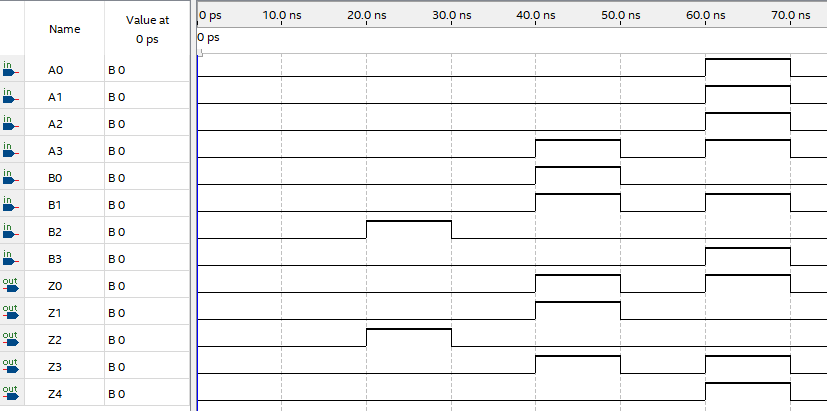
\includegraphics[width=\textwidth]{simulation.png}
    \caption{Simulation results after testing first (0 - 10ns), fifth (20ns - 30ns), tenth (40ns - 50ns), and thirteenth (60ns - 70ns) rows of Table~\ref{table:2}}
    \label{figure:4}
\end{figure}

The simulation yielded \textbf{0b0000 + 0b0000 = 0b00000}, \textbf{0b0000 + 0b0100 = 0b00100}, \textbf{0b1000 + 0b0011 = 0b01011}, \textbf{0b1111 + 0b1010 = 0b11001}, which matched with the corresponding results calculated from Table~\ref{table:2}. We then moved on to real-board testing and also got the same results. Based on the results, we hence believed that our implementations of the 4-bit binary adders were correct.

%%%%%%%%%%%%%%%%%%%%%%%%%%%%%%%%%%%%%%%%%%%%%%%%%%%%%%%%%%%%%%%%%%%%%%%%%%%%%%%%
% Experiment Notes
%%%%%%%%%%%%%%%%%%%%%%%%%%%%%%%%%%%%%%%%%%%%%%%%%%%%%%%%%%%%%%%%%%%%%%%%%%%%%%%%
\section{Experiment Notes}

%%%%%%%%%%%%%%%%%%%%%%%%%%%%%%%%%%%%%%%%
% Reflection
%%%%%%%%%%%%%%%%%%%%%%%%%%%%%%%%%%%%%%%%
\subsection*{Reflection}

This lab brought us from simple schematic design of lab 1 to a more complex design, where we had to define our own ripple-carry adders from scratch (logic gates and wires) and then used the adders in our main circuit. This was quite a big change, but we were able to grasp the idea of reusing sub-circuits and successfully made the grand system work. We are looking forward to more challenging labs in the future.

%%%%%%%%%%%%%%%%%%%%%%%%%%%%%%%%%%%%%%%%
% Study Questions
%%%%%%%%%%%%%%%%%%%%%%%%%%%%%%%%%%%%%%%%
\subsection*{Study Questions}

\begin{enumerate}
    \item Explain how you would convert your 4-bit adder to a 4-bit adder/subtractor.

    \item In your own words, explain what pull resistors do in the FPGA.

    \item Explain your selection for the pullmode for the pin connected to the least-significant full-adder's carry-in.
\end{enumerate}

%%%%%%%%%%%%%%%%%%%%%%%%%%%%%%%%%%%%%%%%%%%%%%%%%%%%%%%%%%%%%%%%%%%%%%%%%%%%%%%%
% Appendix
%%%%%%%%%%%%%%%%%%%%%%%%%%%%%%%%%%%%%%%%%%%%%%%%%%%%%%%%%%%%%%%%%%%%%%%%%%%%%%%%
\section*{Appendix}

No appendix is available in this lab.

\end{document}
